\documentclass{rapport}
\usepackage{lipsum}
\usepackage{gensymb}
\usepackage{float}
\usepackage{graphicx} % Required for inserting images
\usepackage{subcaption}
%\usepackage[demo]{graphicx}
\usepackage{tikz,pgfplots}
\usepackage{amsmath, bm, amssymb,amsfonts,amsthm}
\usepackage{float}
\usepackage[version=4]{mhchem}
\usepackage{siunitx}
\usepackage{longtable,tabularx}
\usepackage{makecell}
\usepackage[labelfont=bf]{caption}
 \usepackage{setspace}
\usepackage[table]{xcolor}
\usepackage[x11names,dvipsnames,table]{xcolor} %for use in color links
\usepackage{colortbl}
\usepackage[utf8]{inputenc}
\usepackage{fontspec}
\usepackage{listings}
\usepackage{xcolor}
\usepackage{booktabs} 

% MATLAB style for listings
\definecolor{darkgreen}{rgb}{0,0.5,0}
\lstset{
  language=Matlab,
  basicstyle=\ttfamily\footnotesize,
  keywordstyle=\color{blue},
  commentstyle=\color{darkgreen},
  stringstyle=\color{red},
  numbers=left,
  numberstyle=\tiny\color{gray},
  stepnumber=1,
  numbersep=5pt,
  backgroundcolor=\color{lightgray!20},
  showspaces=false,
  showstringspaces=false,
  tabsize=4,
  captionpos=b,
  breaklines=true,
  breakatwhitespace=false,
  frame=single
}
% Set font as Calibri
\setmainfont{Carlito}[
    Path=./Carlito/,
    Extension = .ttf,
    UprightFont=*-Regular,
    BoldFont=*-Bold,
    ItalicFont=*-Italic,
    BoldItalicFont=*-BoldItalic
    ]
\title{file title} %title of the file


\begin{document}
%----------- Report information ---------

\logo{Images/logos/nus_logo_full-vertical.jpg}
\uni{\textbf{National University of Singapore\\
EE5114: Autonomous Robot Navigation}}
\ttitle{Localization Using GPS and IMU Information via EKF Framework \\
} %title of the file
\subject{EE5114: Autonomous Robot Navigation} % Subject name

\professor{Dr. Fei \textsc{WANG}} % information related to the professor

\students{Parthiv Vinubhai Kukadia \textsc{(A0304932J)}} % information related to the students

%----------- Init -------------------
        
\buildmargins % display margins
\buildcover % create the front cover of the document

%------------ Report body ----------------

\section{Introduction}
\label{Introduction}
This paper will describe the implementation of coordinate transformation from GPS raw measurement (longitude, latitude, and altitude) to ECEF to NED (x – North, y – East, z – Down) positions with and without a data fusion algorithm – the extended Kalman filter (EKF). The focus of this report is leveraging the EKF to provide a better estimate of the NED positions (in m) and NED velocities (in m/s) by accounting for the difference in update rate between GPS and IMU through manipulating the sensor update frequencies. From the initial code provided and the default plots, it can be deduced that the UAV takes off and lands twice. The total simulation time of the UAV’s flight is 2083 seconds, with the first 32 seconds having irregular data. It takes off the first time at 113 seconds, and lands at 483 seconds. The UAV takes off a 2nd time at 1443 seconds and lands at 1685 seconds. As the report below will show, without implementing an extended Kalman filter (EKF), the estimate of the NED positions is not as accurate and the EKF provides a more accurate state estimate by considering the difference in GPS and IMU update rates and relying on frequent IMU updates for short-term dynamics and less frequent GPS updates for long-term position accuracy. The EKF balances these updates by adjusting the Kalman gain based on the measurement noise and update frequencies. The report will cover the different formulas used to convert from GPS coordinates to NED positions and to implement the extended Kalman filter. It will also provide physical meanings of the state variables and covariance used in EKF, and why specific initialization values were chosen for the states as well as the process and measurement noise covariance, with the respective code.
% instead just say that these questions being answered are xxxx, and this is where you can find it.


\section{Nomenclature}
\label{Nomenclature}
\begin{table}[h!]
\centering
\begin{tabular}{>{\raggedright\arraybackslash}p{8cm} p{8cm}}
\midrule
$a_{cx}$ = x-axis accelerometer reading & $a_{cy}$ = y-axis accelerometer reading \\
$a_{cz}$ = z-axis accelerometer reading & $\Phi$ = Roll angle (phi) \\
$\Theta$ = Pitch angle (theta) & $\Psi$ = Yaw angle (psi) \\
fix = GPS position fix signal & $GPS_{\text{sat}}$ = Number of GPS satellites \\
$eph$ = GPS horizontal variance (m) & $epv$ = GPS vertical variance (m) \\
$lat$ = GPS Latitude & $lat_{\text{ref}}$ = Latitude Reference (initial UAV pos.) \\
$lon$ = GPS Longitude & $lon_{\text{ref}}$ = Longitude Reference (initial UAV pos.) \\
$alt$ = GPS altitude & $alt_{\text{ref}}$ = Altitude Reference (initial UAV pos.) \\
$a$ = Equatorial radius (m) & $b$ = Polar radius (m) \\
$e$ = Eccentricity of ellipsoid & $N$ = Radius of curvature \\
$x_{e0}$ = x-axis ECEF reference pos. & $x_e$ = x-axis ECEF frame \\
$y_{e0}$ = y-axis ECEF reference pos. & $y_e$ = y-axis ECEF frame \\
$z_{e0}$ = z-axis ECEF reference pos. & $z_e$ = z-axis ECEF frame \\
$x_n$ = NED pointing North & $y_n$ = NED pointing East \\
$z_n$ = NED pointing Down & $x$ = State vector $[x,v,b]$ \\
$v_x$ = x-axis velocity NED frame & $v_y$ = y-axis velocity NED frame \\
$v_z$ = z-axis velocity NED frame & $b_x$ = x-axis accelerometer bias \\
$b_y$ = y-axis accelerometer bias & $b_z$ = z-axis accelerometer bias \\
$F$ = State Matrix & $P$ = Covariance matrix \\
$P_0$ = Initial covariance matrix & $u$ = Input vector \\
$G$ = Input Matrix & $y$ = Output vector \\
$H$ = Output (measurement) Matrix & $x_0$ = Initial state vector \\
$\hat{X}$ = State matrix estimate & $Q$ = Process noise covariance matrix \\
$R$ = Measurement noise covariance matrix & $W$ = Optimal Kalman gain matrix \\
$S$ = Innovation covariance matrix & $R_{g/b}$ = Rotation matrix from body to ground frame \\
\bottomrule
\end{tabular}
\end{table}

\section{UAV Take-Off and Landing}
\label{Initial UAV Analysis}
\textbf{By understanding the original codes and observing the default plots of this set of data, can you deduce how many times the UAV had taken off and landed?}
\\

The original code provides data on the accelerometer, Euler angles, GPS, and Motor signals, with plots for each aspect. From observing the default plots, only the motor signal plot provides some sort of understanding of how many times the UAV takes off and lands through the 2 input spikes supplied from the motor - observed over different time intervals. The initial GPS plot shown in Figure. (\ref{fig:GPS Plot}), without any processing, is unclear how often the drone takes off and lands. When analyzing the data on the GPS plots, it can be deduced that in the first 32 seconds of the UAV's flight contains an an anomaly in the data. This anomaly, shown through the spike from around 0 m to 1400 m causes a skew in the plot where you are unable to observe the actual movement of the UAV. From the data provided for the flight time, it is clear that 32 seconds falls at around an index of 125, and therefore, a processed GPS plot (code shown in Figure (\ref{fig:GPS Plot Code})) is created as shown in Figure. (\ref{fig:GPS Plot}), where you can see a more clear view of the flight of the UAV. You are able to tell that the \textbf{UAV takes off two times, the first time it flies up by approximately 10 m (1407 m - 1397 m); the second time it flies up by approximately 31 m (1428 m - 1397 m)}.
\\
\begin{minipage}[H]{0.43\textwidth}
    \centering
    % Insert your graph here
    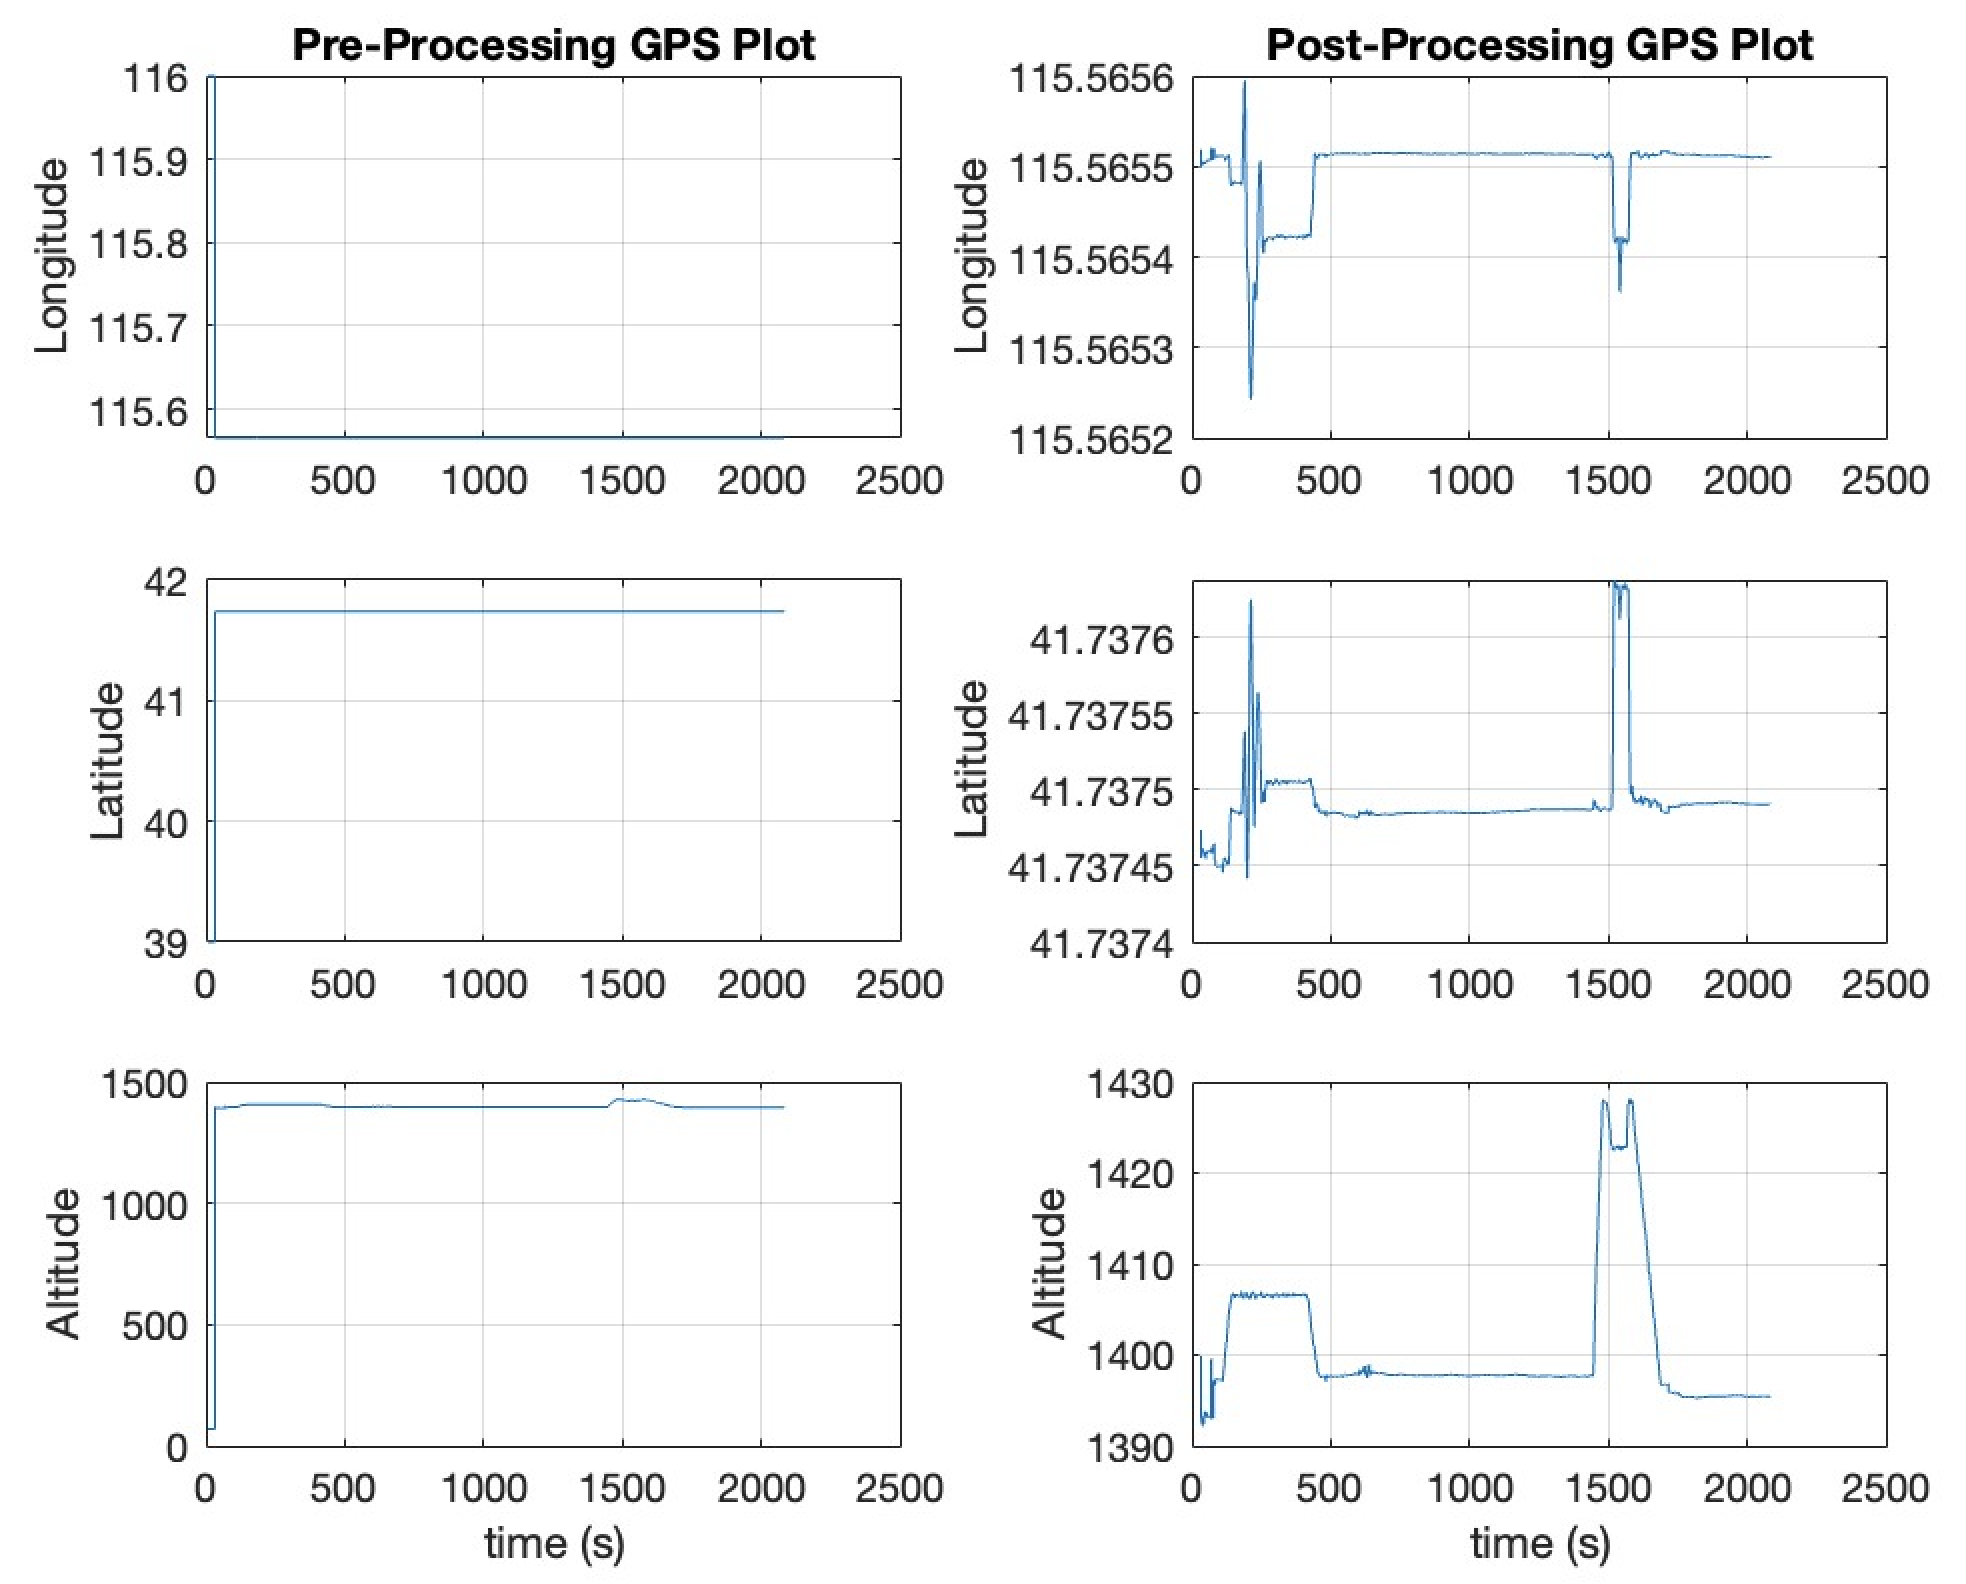
\includegraphics[width=1.6\linewidth]{Introduction/GPS_Plot.png}  
    \label{fig:GPS Plot}
    \captionsetup{justification=centering} % Ensure caption is centered
    \captionof{figure}{Original Code vs. Processed GPS Plot}
\end{minipage}
\hfill
\begin{minipage}{0.3\textwidth}
    \centering
    \lstset{language=Matlab, breaklines=true, basicstyle=\ttfamily\scriptsize}
    \begin{lstlisting}
    
figure; set(gcf,'numbertitle','off','name','GPS');  
subplot(3,2,1); plot(t, lon); title('Pre-Processing GPS Plot'); ylabel('Longitude'); grid on;
subplot(3,2,3); plot(t, lat); ylabel('Latitude'); grid on;
subplot(3,2,5); plot(t, alt); ylabel('Altitude'); grid on; xlabel('time (s)');
subplot(3,2,2); plot(t(125:end), lon(125:end)); title('Post-Processing GPS Plot'); ylabel('Longitude'); grid on;
subplot(3,2,4); plot(t(125:end), lat(125:end)); ylabel('Latitude'); grid on;
subplot(3,2,6); plot(t(125:end), alt(125:end)); ylabel('Altitude'); grid on; xlabel('time (s)');
    \end{lstlisting}
    \captionof{figure}{MATLAB Code for Processed GPS Plot}
    \label{fig:GPS Plot Code}
\end{minipage}


\textbf{}
\\
\textbf{When did the UAV take off and land the second time?}
\\

From Figure. (\ref{fig:GPS Plot}), we can see that the UAV took off the first time at about 113 seconds from when data started to be collected. It was in flight for about 370 seconds, during which point, at 483 seconds, it returned to the base altitude of the UAV of 1397.8 m. \textbf{The UAV took off a second time at about 1443 seconds (24 minutes into flight data being tracked) and was in flight for about 242 seconds when it came back to the base altitude of the UAV at 1685 seconds (28 minutes into flight data being tracked).} The resting state of the UAV can be seen to be at an altitude of around 1397.8 m, which we will take as the UAV being on the ground. Using 1397.8 m as the ground frame measurement, we can capture the time the UAV takes off and lands when we see the base of the 2 spikes in the post-processed altitude graph and the flat line for when the curve returns to our assumed ground frame measurement.


\section{GPS Raw Measurements to NED Positions}
\label{GPStoNED}
\textbf{List the formulas you have used to convert GPS coordinates to NED positions and attach your corresponding codes for this step.}\\

To convert from GPS coordinates to NED positions, it is required that you convert from Geodetic coordinate frame $ [longitude ($\lambda$), latitude ($\phi$), altitude (h)]^T$ to Earth-Centered, Earth Fixed (ECEF) coordinate frame $[$x_e$, $y_e$, $z_e$]^T$ to North-East-Down (NED) coordinate frame $[$x_n$, $y_n$, $z_n$]^T$. \\
To Convert from Geodetic to ECEF, you need to define Earth's Equatorial radius (a), Earth's Polar radius (b), which can then be used to calculate the eccentricity of the Earth ellipsoid (e). These variables are used to define the Prime vertical radius of curvature N($\varphi$). The equations shown in Eq.(\ref{Geo2ECEF}) will be used to compute the ECEF coordinates.

\begin{equation}
\begin{aligned}
X_e &= \left(N(\varphi) + h\right) \cos \varphi \cos \lambda\\
Y_e &= \left(N(\varphi) + h\right) \cos \varphi \sin \lambda\\
Z_e &= \left(\frac{b^2}{a^2} N(\varphi) + h \right) \sin \varphi
\end{aligned}
\label{Geo2ECEF}
\end{equation}

where
\begin{equation}
N(\varphi) = \frac{a^2}{\sqrt{a^2 \cos^2 \varphi + b^2 \sin^2 \varphi}} = \frac{a^2}{\sqrt{1 - e^2 \sin^2 \varphi}}
\label{N_phi}
\end{equation} \\

You begin by converting the latitude, and longitude to radians, since they are provided to us in degrees. The size of the latitude, longitude, altitude, and time vectors are 10215 x 1, so the converted latitude and longitude in radians will also be a 10215 x 1 vector. The first step now will be to define the initial UAV position as the reference position being used for the coordinate transformation. This initial position will be the first input in the data set at time index = 1. By defining the reference latitude and longitude, it is possible to now calculate the initial ECEF coordinate frame position $[$x_(e0)$, $y_(e0)$, $z_(e0)$]^T$. Using Eq.(\ref{Geo2ECEF}), the ECEF coordinates are calculated for each time index using a for-loop.
\\
\\
After calculating the initial ECEF position and the ECEF positions as a 10215 x 3 matrix, the next step is to calculate the NED positions. To calculate the local NED coordinates from ECEF, you need to apply a rotation matrix to the difference between the ECEF position at that point in time and the reference point in ECEF coordinates, as shown in Eq.(\ref{ECEF2NED}).

\begin{equation}
\begin{bmatrix}
X_n \\
Y_n \\
Z_n
\end{bmatrix}
=
R^T
\left(
\begin{bmatrix}
X_e \\
Y_e \\
Z_e
\end{bmatrix}
-
\begin{bmatrix}
X_{e0} \\
Y_{e0} \\
Z_{e0}
\end{bmatrix}
\right)
\label{ECEF2NED}
\end{equation}

where

\begin{equation}
R =
\begin{bmatrix}
-\sin \varphi \cos \lambda & -\sin \lambda & -\cos \varphi \cos \lambda \\
-\sin \varphi \sin \lambda & \cos \lambda & -\cos \varphi \sin \lambda \\
\cos \varphi & 0 & -\sin \varphi
\end{bmatrix}
\end{equation}
\\
For each NED coordinate, you substitute the ECEF coordinate and the respective latitude and longitude values in radians into the rotation matrix to get the NED positions at that time index. Creating a for-loop allows you to get the respective NED coordinates in a 10215 x 3 matrix for the x, y, and z coordinates. For this transformation, 3 functions were created as shown in Fig (\ref{fig:GPS2NEDMatlab}), where 1 function converts GPS to ECEF, 1 converts ECEF to NED, and then a master function that houses the 2 functions to convert each GPS raw measurement to a local NED position. The graph obtained for the NED positions from the coordinate transformation can be seen below, where similar to the GPS plot, we eliminate the first 32 seconds of the data to remove the irregularity in the data set to provide us a more accurate graph.

\begin{figure}[H]
  \centering
 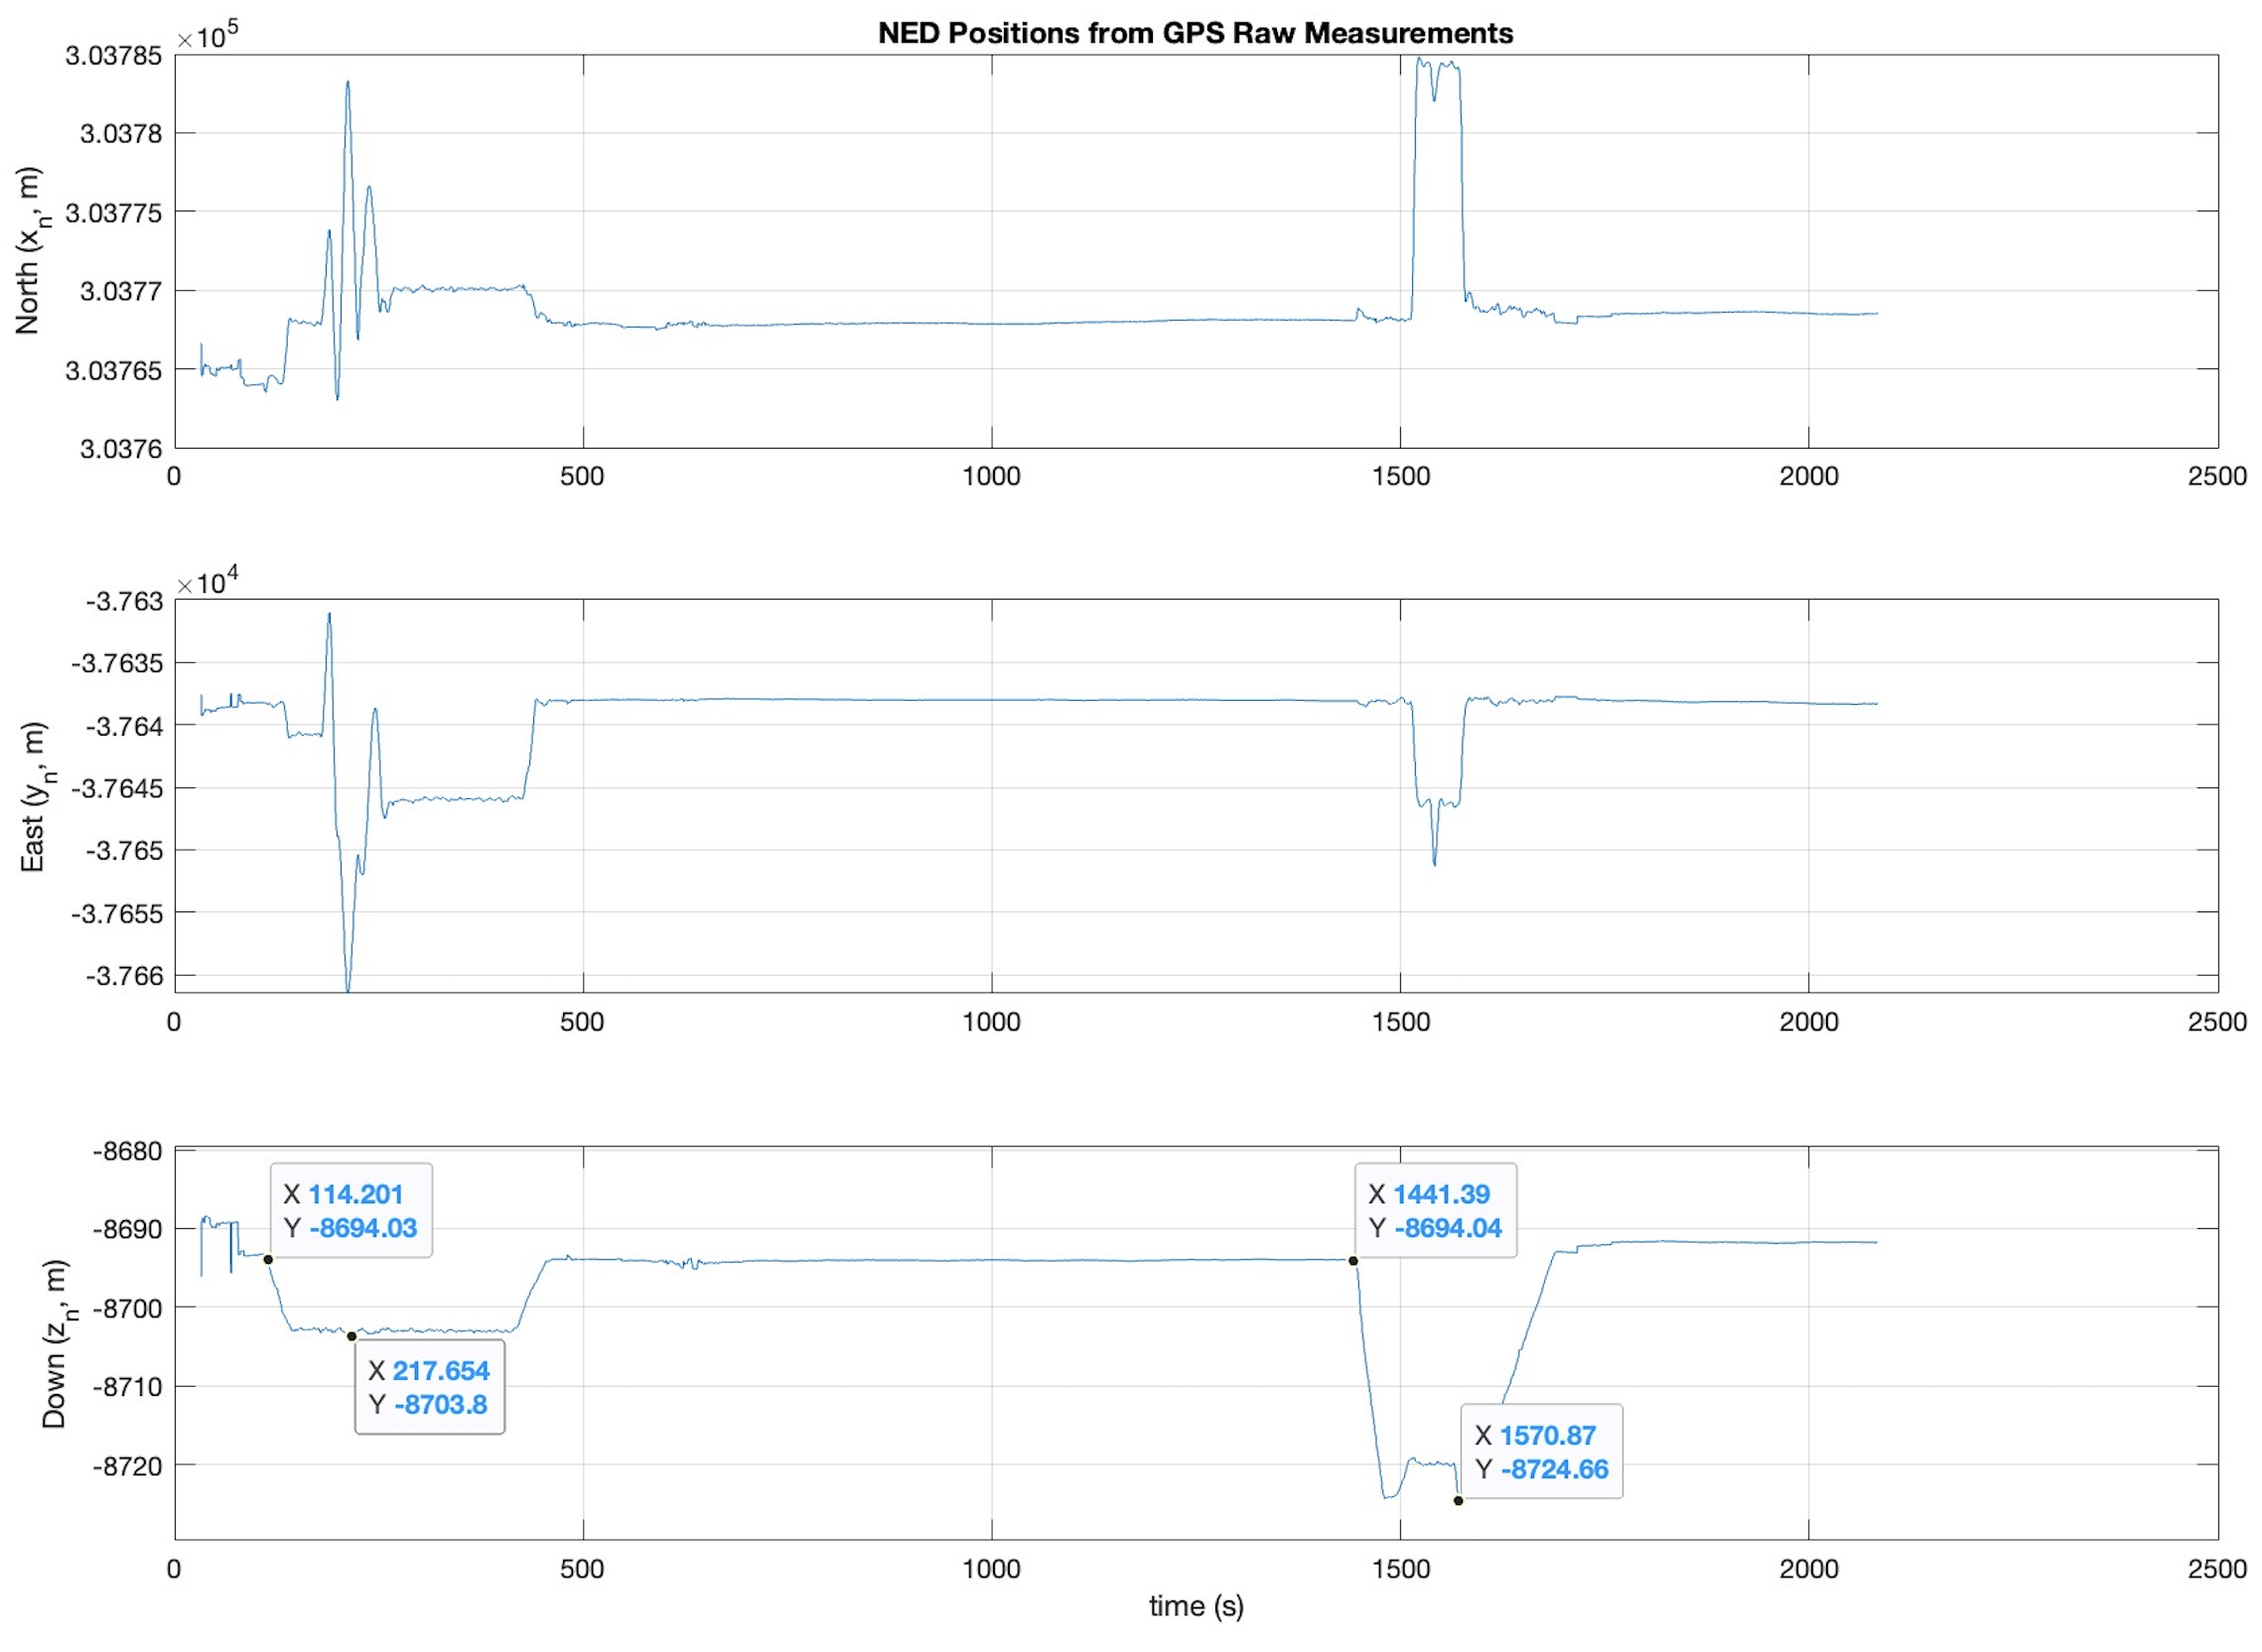
\includegraphics[width=0.8\linewidth, height=0.7\linewidth]{GPS/GPS2NED.png}  
\caption{NED Positions from GPS Raw Measurements}
\label{fig:GPS2NED}
\end{figure}
\\
As the graph in Fig (\ref{fig:GPS2NED}) shows, the UAV takes off twice at the same time frame as the GPS plot. From analyzing the graph, the data shows that during the first UAV take-off and landing, it flies about 10 m (8704 m (max height) - 8694 m ("zero" height)). During the second UAV take-off and landing, it flies approximately 31 m (8725 m (max height) - 8694 m ("zero" height)). The NED positions are validated from the GPS data, showing that the GPS raw measurement to local NED position is completed with great accuracy. We see that the Down ($z_n$ graph is flipped from the GPS Plot, and that is because of the way the axis is defined, but the magnitude of the altitude change for both the GPS plot and the NED positions plot validates the transformation. The code for the transformation from GPS to NED can be found in Fig. (\ref{GPStoNED Matlab Code}). 

\label{GPStoNED Matlab Code}
\begin{lstlisting}
% To obtain local NED from GPS, need to convert Geodetic to ECEF to NED coordinate frame.

% Convert Latitude and Longitude to Radians
lat_rad = deg2rad(lat);
lon_rad = deg2rad(lon);

% Create a function to convert GPS to NED coordinate Frame
function [NED_Coordinates] = GPStoNED(lat_rad, lon_rad, alt)
    % Constants for Earth Ellipsoid to convert from Geodetic to ECEF
    a = 6378137;
    b = 6356752.3142;
    e2 = 1 - (b^2 / a^2);
    % Define initial UAV position as reference position
    lat_0 = lat_rad(1); % Reference Latitude
    lon_0 = lon_rad(1); % Reference Longitude
    alt_0 = alt(1); % Reference Altitude
    % Convert defined intial GPS reference position to ECEF coordinate frame
    [x_e0, y_e0, z_e0] = GPStoECEF(lat_0, lon_0, alt_0, a, e2);
    % Create arrays for NED Coordinates to be stored after iteration
    NED_Coordinates = zeros(length(lat_rad), 3);
    % Loop over all GPS raw measurements and convert each to NED coordinates
    for i = 1:length(lat_rad)
        % Convert GPS raw measurements to ECEF coordinate frame
        [x_e, y_e, z_e] = GPStoECEF(lat_rad(i), lon_rad(i), alt(i), a, e2);
        % Convert ECEF measurements to NED coordinate frame
        [x_n, y_n, z_n] = ECEFtoNED(x_e, y_e, z_e, x_e0, y_e0, z_e0, lat_rad(i), lon_rad(I));
        % Store NED coordinates in created arrays
        NED_Coordinates(i, :) = [x_n, y_n, z_n];
    end
end

% Create a function to convert GPS to ECEF coordinate frame
function [x_e, y_e, z_e] = GPStoECEF(lat, lon, alt, a, e2)
    % Define radius of curvature
    N = a ./ sqrt(1 - e2 .* sin(lat).^2); % Radius of curvature
    % Convert GPS raw measurements to ECEF coordinate frame
    x_e = (N + alt) .* cos(lat) .* cos(lon);
    y_e = (N + alt) .* cos(lat) .* sin(lon);
    z_e = ((1 - e2) .* N + alt) .* sin(lat);
end

% Create a function to convert ECEF to NED coordinate frame
function [x_n, y_n, z_n] = ECEFtoNED(x_e, y_e, z_e, x_e0, y_e0, z_e0, lat, lon)
    % Difference between ECEF current coordinate and ECEF reference point
    dx = x_e - x_e0;
    dy = y_e - y_e0;
    dz = z_e - z_e0;
    % Rotation matrix to go from ECEF to NED coordinate system
    R = [-sin(lat) * cos(lon), -sin(lon) , -cos(lat) * cos(lon) ;
         -sin(lat) * sin(lon), cos(lon)  , -cos(lat) * sin(lon) ;
         cos(lat)            ,     0     , -sin(lat)           ];
    % Calculate NED coordinates
    NED = R' * [dx; dy; dz];
    x_n = NED(1); y_n = NED(2); z_n = NED(3);
end

% Run the NED_Coordinates function to compute a GPS to NED Coordinate
% Transform and substitute into correct naming convention [x_n, y_n, z_n]
[NED_coords] = GPStoNED(lat_rad, lon_rad, alt);
x_n = NED_coords(:,1); y_n = NED_coords(:,2); z_n = NED_coords(:,3);

%% GPS to NED Plot
figure; set(gcf,'numbertitle','off','name','NED Positions from GPS Raw Measurements');  
subplot(3,1,1); plot(t(125:end), x_n(125:end));title('NED Positions from GPS Raw Measurements'); ylabel('North (x_n, m)'); grid on;
subplot(3,1,2); plot(t(125:end), y_n(125:end)); ylabel('East (y_n, m)'); grid on;
subplot(3,1,3); plot(t(125:end), z_n(125:end)); ylabel('Down (z_n, m)'); grid on; xlabel('time (s)');
\end{lstlisting}
\captionof{figure}{MATLAB Code for GPS Raw Measurement to Local NED Positions}
\label{fig:GPS2NEDMatlab}


\section{Implementing Extended Kalman Filter for Estimated NED Position and Velocity}
\label{EKF}
\textbf{List the formulas you have used for the implementation of Kalman filter}\\

Implementing the extended Kalman filter for this simulation is to be done on a specific time frame of the UAV's flight - 10 minutes before the 2nd time the UAV takes off and 5 minutes after the UAV lands the 2nd time. For this time interval, begin by defining a start time (1443 seconds - 600 seconds) and an end time (1685 seconds + 300 seconds). Once this time is defined, identify the index within the time inputs to understand what index Matlab needs to begin implementing the EKF and what index it needs to stop. This is the first step in implementing the EKF.\\
To Implement an Extended Kalman Filter, begin by defining the initial state variables, the initial state covariance matrix (P), and the Measurement Covariance matrix (R):
\subsection*{State Variables}

\[
x_0 = 
\begin{bmatrix}
x_n \\
y_n \\
z_n \\
v_{x} \\
v_{y} \\
v_{z} \\
b_x \\
b_y \\
b_z
\end{bmatrix}
=
\begin{bmatrix}
x_n (@start_{time} index) \\
y_n (@start_{time} index) \\
z_n (@start_{time} index) \\
0 \\
0 \\
0 \\
0 \\
0 \\
0
\end{bmatrix}
\]\\
\textbf{Please explain the physical meanings of your state variables used in your EKF and which coordinate system they are defined in. }\\

Where $x_n$, $y_n$ and $z_n$ are the NED position coordinates, $v_x$, $v_y$, $v_z$ are the velocities of the UAV also in the NED frame, and $b_x$, $b_y$, $b_z$ are the accelerometer bias provided in the body frame.

\subsection*{State Covariance (P Matrix)}

\[
P =
\begin{bmatrix}
P_{xx} & P_{xy} & P_{xz} & P_{xv_x} & P_{xv_y} & P_{xv_z} & P_{xb_x} & P_{xb_y} & P_{xb_z} \\
P_{yx} & P_{yy} & P_{yz} & P_{yv_x} & P_{yv_y} & P_{yv_z} & P_{yb_x} & P_{yb_y} & P_{yb_z} \\
P_{zx} & P_{zy} & P_{zz} & P_{zv_x} & P_{zv_y} & P_{zv_z} & P_{zb_x} & P_{zb_y} & P_{zb_z} \\
P_{v_xx} & P_{v_xy} & P_{v_xz} & P_{v_xv_x} & P_{v_xv_y} & P_{v_xv_z} & P_{v_xb_x} & P_{v_xb_y} & P_{v_xb_z} \\
P_{v_yx} & P_{v_yy} & P_{v_yz} & P_{v_yv_x} & P_{v_yv_y} & P_{v_yv_z} & P_{v_yb_x} & P_{v_yb_y} & P_{v_yb_z} \\
P_{v_zx} & P_{v_zy} & P_{v_zz} & P_{v_zv_x} & P_{v_zv_y} & P_{v_zv_z} & P_{v_zb_x} & P_{v_zb_y} & P_{v_zb_z} \\
P_{b_xx} & P_{b_xy} & P_{b_xz} & P_{b_xv_x} & P_{b_xv_y} & P_{b_xv_z} & P_{b_xb_x} & P_{b_xb_y} & P_{b_xb_z} \\
P_{b_yx} & P_{b_yy} & P_{b_yz} & P_{b_yv_x} & P_{b_yv_y} & P_{b_yv_z} & P_{b_yb_x} & P_{b_yb_y} & P_{b_yb_z} \\
P_{b_zx} & P_{b_zy} & P_{b_zz} & P_{b_zv_x} & P_{b_zv_y} & P_{b_zv_z} & P_{b_zb_x} & P_{b_zb_y} & P_{b_zb_z}
\end{bmatrix}
= I_{9x9} (9x9 Identity Matrix)
\]\\

\textbf{Please explain what values you have chosen to initialize the state variables and the state covariance matrix P. Why these values?}\\

The state variables have been initialized with the first value of the NED positions at the provided start time, since that is what the EKF implementation required (for the UAV being 10 minutes before taking off), and therefore, using the index created with the time, we can implement that start index to capture the initial NED position of the UAV for our initial state vector. The velocities are initialized at 0 to assume that the UAV is beginning at a stationary flight, with the velocity incrementally updating through implementing EKF using accelerometer readings. If the velocity was initialized incorrectly, the beauty of EKF is that it would adjust the velocity estimates based on subsequent readings. The accelerometer bias was initialized with 0's as well since the initial bias is unknown and it is common practice to set the values to 0 and let the EKF estimate it over its iterations since the EKF will cause the bias to converge over time to the correct estimate of the bias based on the sensor readings. As more data is provided from the IMU and the GPS, the filter will help adjust the bias estimates to provide a more accurate value for the accelerometer bias, which we will show through a plot. For the state covariance, we initialize the data as a 9x9 identity matrix, with a weight of 1 provided for the diagonals of P, which is the uncertainty of each state variable ($P_{xx}, P_{yy}, P_{zz}, P_{vxvx}, P_{vyvy}, P_{vzvz}, P_{bxbx}, P_{byby}, P_{bzbz}$, where the diagonals of the P matrix = the variance of each state, and the non-diagonals = covariance. With a weight of 1, we begin by telling the system that there is a moderate degree of uncertainty for each state variable and this uncertainty is the same - a neutral, non-bias assumption of uncertainty.\\

Now, the process requires the system to be defined that we will implement EKF on to estimate the NED Position and Velocity.
\subsection*{System:}

\begin{align}
    \mathbf{x}(k+1) &= F\mathbf{x}(k) + G\mathbf{u}(k) + \mathbf{v}(k) \\
    \mathbf{y}(k) &= H\mathbf{x}(k) + \mathbf{w}(k)
\end{align}
Where the respective matrices can be computed using the process model shown below:

\subsection*{Process Model (works for navigation within small earth surface area)}

\[
\begin{bmatrix}
x \\
y \\
z \\
v_x \\
v_y \\
v_z \\
b_x \\
b_y \\
b_z
\end{bmatrix}_{k+1}
=
\underbrace{
\begin{bmatrix}
1 & 0 & 0 & dt & 0 & 0 & -dt^2/2 & 0 & 0 \\
0 & 1 & 0 & 0 & dt & 0 & 0 & -dt^2/2 & 0 \\
0 & 0 & 1 & 0 & 0 & dt & 0 & 0 & -dt^2/2 \\
0 & 0 & 0 & 1 & 0 & 0 & -dt & 0 & 0 \\
0 & 0 & 0 & 0 & 1 & 0 & 0 & -dt & 0 \\
0 & 0 & 0 & 0 & 0 & 1 & 0 & 0 & -dt \\
0 & 0 & 0 & 0 & 0 & 0 & 1 & 0 & 0 \\
0 & 0 & 0 & 0 & 0 & 0 & 0 & 1 & 0 \\
0 & 0 & 0 & 0 & 0 & 0 & 0 & 0 & 1
\end{bmatrix}
}_{F}
\begin{bmatrix}
x \\
y \\
z \\
v_x \\
v_y \\
v_z \\
b_x \\
b_y \\
b_z
\end{bmatrix}_k
+
\underbrace{
\begin{bmatrix}
\frac{dt^2}{2} & 0 & 0 \\
0 & \frac{dt^2}{2} & 0 \\
0 & 0 & \frac{dt^2}{2} \\
dt & 0 & 0 \\
0 & dt & 0 \\
0 & 0 & dt \\
0 & 0 & 0 \\
0 & 0 & 0 \\
0 & 0 & 0 
\end{bmatrix}
}_{G}
\begin{bmatrix}
R_{g/b} \\
0 \\
g
\end{bmatrix}
\begin{bmatrix}
a_x \\
a_y \\
a_z \\
1
\end{bmatrix}_k
\]

Where $(R_{g/b})$ is a rotation matrix to convert the values from the body frame to the ground frame.

\[
R_{g/b} = 
\begin{pmatrix}
\dot{X}_n \\
\dot{Y}_n \\
\dot{Z}_n
\end{pmatrix}
=
\begin{bmatrix}
c_\psi c_\theta & c_\psi s_\theta s_\phi - s_\psi c_\phi & c_\psi s_\theta c_\phi + s_\psi s_\phi \\
s_\psi c_\theta & s_\psi s_\theta s_\phi + c_\psi c_\phi & s_\psi s_\theta c_\phi - c_\psi s_\phi \\
-s_\theta       & c_\theta s_\phi                         & c_\theta c_\phi
\end{bmatrix}
\begin{pmatrix}
u \\
v \\
w
\end{pmatrix}
\]

\subsection*{Process Noise Covariance}

\[
Q = G
\begin{bmatrix}
q_x & 0 & 0 & 0 \\
0 & q_y & 0 & 0 \\
0 & 0 & q_z & 0 \\
0 & 0 & 0 & 0
\end{bmatrix}
G' = 
G
\begin{bmatrix}
0.7 & 0 & 0 & 0 \\
0 & 0.4 & 0 & 0 \\
0 & 0 & 1.5 & 0 \\
0 & 0 & 0 & 0
\end{bmatrix}
G'
\]

\subsection*{Measurement Noise Covariance (R Matrix)}

\[
R =
\begin{bmatrix}
R_{xx} & 0      & 0      \\
0      & R_{yy} & 0      \\
0      & 0      & R_{zz}
\end{bmatrix}
= 
\begin{bmatrix}
eph & 0      & 0      \\
0      & eph & 0      \\
0      & 0      & epv
\end{bmatrix} * 1e-3
\]

\subsubsection*{1. Predict}

\begin{align}
    \hat{\mathbf{x}}(k+1 | k) &= F \hat{\mathbf{x}}(k | k) + G\mathbf{u}(k) \\
    P(k+1 | k) &= F P(k | k) F^T + Q
\end{align}

\subsubsection*{2. Correction}

\begin{align}
    S &= H P(k+1 | k) H^T + R \\
    W &= P(k+1 | k) H^T S^{-1} \\
    \Delta \mathbf{x} &= W \left( \mathbf{y}(k+1) - H \hat{\mathbf{x}}(k+1 | k) \right)
\end{align}

\subsubsection*{3. Update}

\begin{align}
    \hat{\mathbf{x}}(k+1 | k+1) &= \hat{\mathbf{x}}(k+1 | k) + W \mathbf{v} \\
    P(k+1 | k+1) &= P(k+1 | k) - W S W^T
\end{align}
Where H is the measurement matrix relating the state vector to the measurements, mapping the state space to the measurement space. The matrix H in our system is given by:
\begin{align*}
    H = \begin{bmatrix}
    1 & 0 & 0 & 0 & 0 & 0 & 0 & 0 & 0 \\
    0 & 1 & 0 & 0 & 0 & 0 & 0 & 0 & 0 \\
    0 & 0 & 1 & 0 & 0 & 0 & 0 & 0 & 0
    \end{bmatrix}
\end{align*}

\textbf{Explain the choice of Q and R matrices for EKF implementation.}\\

Initially, I defined the Q matrix with 1's in the $q_x, q_y, q_z$ diagonals, and the R matrix to be the horizontal and vertical variance from the GPS since GPS measurements are the most accurate. Using these initial values of Q and R, I defined the process and implemented the EKF using just GPS readings to see if my Q and R matrix of the model was accurate. The first attempt showed that there was a lot of drift in my EKF estimated position, as well as velocity. Therefore I knew that I had to tune my Q and R matrix to allow my EKF estimation to better match my NED positions from GPS raw measurements. The tuning process for both Q and R were a little different since each matrix affected the system differently. I started by focusing on Q. The Q matrix - process noise covariance supports the system by defining the uncertainty in the IMU measurements from the accelerometer. Theoretically, if the weight on Q was too large, EKF would result in trusting the IMU readings more than it should, resulting in a greater drift, and if the value was too small, then the GPS readings would be trusted more, producing greater noise in the system. Therefore, knowing that GPS was the most accurate reading I had, I reduced my Q from 1's to decimals (i.e., 0.7, 0.4, 1.5), which provided a more accurate estimation from EKF to the GPS to NED measurements. Once I was able to tune Q, it was time to focus on R - the measurement noise covariance. R is used to define the uncertainty present in our GPS data, which means that the more noisy the GPS data is, the better R can help in reflecting the actual noise characteristics of GPS. Theoretically, increasing R would result in EKF not trusting GPS measurements as much, and reducing R would cause the system to trust the noisy GPS data more. Therefore, from trial and error of different values, I was able to capture an R matrix that better estimated my NED position with the GPS horizontal and vertical covariance values being reduced by 1e-3.\\

Once I was able to define a Q and R matrix that was able to estimate NED position and velocity accurately, I could address the issue of the difference in GPS and IMU update rates.\\

\textbf{GPS update rate is slower than IMU update rate, explain how you implemented code to address this practical issue.}\\

Since the GPS update rate is slower than the IMU update rate, I decided to not take all GPS inputs to update the prediction step of the NED position estimate and to instead use a time gap (i.e., take fewer GPS inputs to allow for correction and update step to match IMU better). This time gap was selected to be every 2nd GPS input for 1 IMU update (e.g., 1st update step using IMU, 2nd update step comes from correction step with GPS update, and then an update step using GPS). The value of using every 2nd GPS input vs. 5th or 10th was done using an iterative process, where the process began without skipping some GPS values (i.e, mod (i,1) == 0) to see the estimation of NED positions implementing EKF. From skipping no values, we iterated by increasing the # of GPS inputs being skipped up until 10. As the # of inputs being skipped increased over 4, the estimation started to produce a larger drift for the NED positions. This resulted in the final implementation to capture every 2nd GPS input into correction and update step of the EKF implementation to produce the figure shown below.\\
This implementation of not updating every prediction value using GPS input allowed to estimate the NED positions with more accuracy as shown in the plot below. It is visible that EKF implementation (shown through the Black line) is mimicking the NED positions from GPS (shown through the dotted red line). 

\begin{figure}[H]
  \centering
 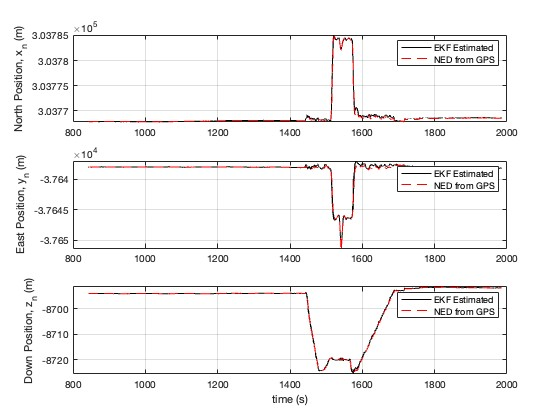
\includegraphics[width=0.8\linewidth, height=0.7\linewidth]{EKF/EKF_Pos.jpg}  
\caption{NED Positions Estimated from EKF Implementation}
\label{fig:EKFPos}
\end{figure}
\\
Since the state estimate also provided us with velocity and acceleration bias, to compare the velocity from the GPS-derived NED positions, we differentiated the NED positions from raw GPS measurement. First, define the time derivative $dt_v$ which is the derivative of the time-interval for the UAV's 2nd flight, which was 10 minutes before taking off and 5 minutes after landing. To calculate the velocity, we differentiate the NED positions from the start-to-end index defined for our EKF implementation and we divide it by $dt_v$.
\begin{align*}
    \Delta t_v &= \text{diff}( \text{time\_int} ) \\
    v_n &= \frac{\text{diff}(x_n( \text{start\_i} : \text{end\_i}))}{\Delta t_v} \\
    v_e &= \frac{\text{diff}(y_n( \text{start\_i} : \text{end\_i}))}{\Delta t_v} \\
    v_d &= \frac{\text{diff}(z_n( \text{start\_i} : \text{end\_i}))}{\Delta t_v} \\
\end{align*}\\
Since the Velocity of the UAV from NED was captured through differentiating the NED positions, the EKF estimation of velocity uses both IMU data and GPS data to estimate velocity, while accounting for sensor noise and drift. It filters the noise through using the process model and Kalman gain, allowing an estimation of a smoother and less noisy velocity estimate in comparison to the differentiated NED position - velocity. Since the EKF incorporates bias correction, the EKF is able to correct the velocity estimate based on accelerometer bias over time allowing it to reduce the impact of the sensor's drift on the estimated velocity, providing a more accurate velocity reading. NED-differentiated velocity is more accurate when the GPS data is more frequent and with minimal noise, but when the motion is fast or involves frequent changes in velocity, the EKF is more accurate due to the high IMU update rate. In our case, the EKF estimated velocity is more accurate and can be seen from the graph below.

\begin{figure}[H]
  \centering
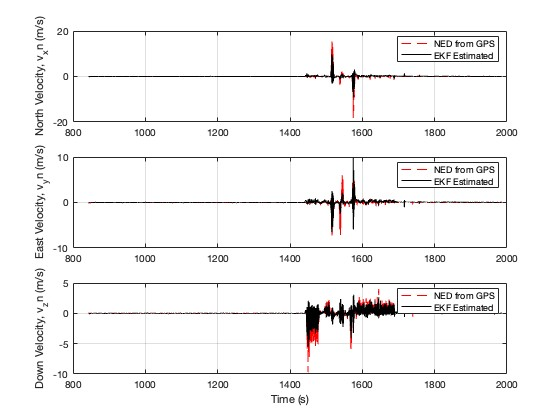
\includegraphics[width=0.8\linewidth, height=0.7\linewidth]{EKF/EKF_Vel.jpg}  
\caption{NED Velocity Estimated from EKF Implementation}
\label{fig:EKFVel}
\end{figure}

You can find below the code used to implement EKF and produce the necessary graphs in section 5, Implementing Extended Kalman Filter for NED Position and Velocity.
\label{EKF Estimated NED Matlab Code}
\begin{lstlisting}
% Implementing EKF for time 2nd UAV take-off and landing where t_min is 10 minutes before UAV taking off and t_max is 5 minutes after landing. From Motor Signal, we can see that UAV took off at 1440 seconds, and landed at 1695 seconds

% Define time interval as provided in the problem statement and define time index to synchronize data between GPS and IMU to align readings based on timestamp
start_t = 1443 - 600; % 10 min before taking-off a second time
start_i = find(t>= start_t,1); % Start time index
end_t = 1685 + 300; % 5 min after landing a second time
end_i = find(t>= end_t,1); % End time index
time_int = t(start_i:end_i); % Define time values from time dataset

% State Variables of interest [NED Position, NED Velocity, Accelerometer Bias]
% x = [x_n, y_n, z_n, v_x, v_y, v_z, b_x, b_y, b_z]
% Define initial state, covariance, and measurement noise covariance
x0 = [x_n(start_i); y_n(start_i); z_n(start_i); 0; 0; 0; 0; 0; 0]; % State
P0 = eye(9); % Covariance
R = diag([eph,eph,epv]) * 1e-3; % Measurement noise covariance, GPS is most reliable
x_hat = zeros(9, length(time_int)); % Create arrays for NED estimate coordinates

% Implementing Extended Kalman Filter - Create System Matrices
for i = start_i:end_i
    dt = (time_int(end) - time_int(1))/(length(time_int)); % Assuming uniform sampling

    % Create Rotation Matrix to move from NED to Ground Frame
    R_NEDtoGround = [cos(psi(i)) * cos(tht(i)) , (cos(psi(i)) * sin(tht(i)) * sin(phi(i))) - (sin(psi(i)) * cos(phi(i))) , (cos(psi(i)) * sin(tht(i)) * cos(phi(i))) + (sin(psi(i)) * sin(phi(i)));
    sin(psi(i)) * cos(tht(i)) , (sin(psi(i)) * sin(tht(i)) * sin(phi(i))) + (cos(psi(i)) * cos(phi(i))) , (sin(psi(i)) * sin(tht(i)) * cos(phi(i))) - (cos(psi(i)) * sin(phi(i)));
    -sin(tht(i)),  cos(tht(i)) * sin(phi(i)),  cos(tht(i)) * cos(phi(i))];
    
    % Create the State Transition Matrix
    F_1 = [eye(3), diag([dt, dt, dt]) , diag([(-dt^2)/2, (-dt^2)/2, (-dt^2)/2]); 
           zeros(3,3) , eye(3), diag([-dt, -dt, -dt])];
    F_2 = [eye(6), zeros(6,3);
           zeros(3,6) , R_NEDtoGround];
    F = [F_1 * F_2         ;  % Upper region of F
         zeros(3,6), eye(3)]; % Lower region of F

    % Define gravity for G matrix
    g = 9.81; % m/s^2

    % Create the Control Input Matrix
    G_1 = [diag([(dt^2)/2, (dt^2)/2 , (dt^2)/2]);
           diag([  dt    ,    dt    ,   dt    ]);
                          zeros(3,3)           ];
    G_2 = [R_NEDtoGround, [0 ; 0 ; g]];
    G = G_1 * G_2;

    % Create process noise covariance matrix
    Q = G * diag([0.7 , 0.4 , 1.5 , 0]) * G'; %qx, qy, qz

    % Prediction Step - using the previous time step to produce an estimation of the state at the current time step
    x_pred = (F * x0) + (G * [acx(i) ; acy(i) ; acz(i) ; 1]);
    P_pred = (F * P0 * F') + Q;

    % Defining the Measurement Model of GPS
    y = [x_n(i+1) ; y_n(i+1) ; z_n(i+1)];

    % To account for the difference in GPS update rate and IMU update rate, need to input a condition such that the GPS update rate is lower to provide long-term position accuracy
    if mod(i, 2) == 0
        % Correction Step with GPS update (every 3rd iteration)
        H = [eye(3), zeros(3, 6)]; % Output Matrix
        S = (H * P_pred * H') + R; % Residual covariance
        W = P_pred * H' * inv(S);  % Optimal Kalman Gain

        % Update step using GPS
        x0 = x_pred + (W * (y - (H * x_pred)));
        P0 = (eye(9) - (W * H)) * P_pred;
        
    else
        % Update step without GPS (IMU update)
        x0 = x_pred;
        P0 = P_pred;
    end

    % Store estimates
    x_hat(:,i) = x0;
end   

% Extract estimated velocities
x_hat = x_hat(:,start_i:end_i);
EKF_pos_N = x_hat(1, :); EKF_pos_E = x_hat(2, :); EKF_pos_D = x_hat(3, :);
EKF_vel_N = x_hat(4, :); EKF_vel_E = x_hat(5, :); EKF_vel_D = x_hat(6, :);
EKF_bx = x_hat(7, :); EKF_by = x_hat(8, :); EKF_bz = x_hat(9, :);

% Calculate NED Velocity and Acceleration from GPS Measurement
dt_v = diff(time_int); dt_a = diff(dt_v);
v_n = diff(x_n(start_i:end_i))./dt_v; a_n = diff(v_n)./dt_a;
v_e = diff(y_n(start_i:end_i))./dt_v; a_e = diff(v_e)./dt_a;
v_d = diff(z_n(start_i:end_i))./dt_v; a_d = diff(v_d)./dt_a;

%% Plot of estimated NED positions based on EKF vs. time
figure; set(gcf,'numbertitle','off','name','EKF Estimated NED Positions');  
subplot(3,1,1); plot(time_int, EKF_pos_N, 'k', time_int, x_n(start_i:end_i), 'r--' ); legend('EKF Estimated', 'NED from GPS');ylabel('North Position, x_n (m)'); grid on;
subplot(3,1,2); plot(time_int, EKF_pos_E, 'k', time_int, y_n(start_i:end_i), 'r--' ); legend('EKF Estimated', 'NED from GPS');ylabel('East Position, y_n (m)'); grid on;
subplot(3,1,3); plot(time_int, EKF_pos_D, 'k', time_int, z_n(start_i:end_i), 'r--' ); legend('EKF Estimated', 'NED from GPS');ylabel('Down Position, z_n (m)'); grid on; xlabel('time (s)');

%% Estimated NED velocities based on EKF Implementation againt time
figure; set(gcf,'numbertitle','off','name','EKF Estimated NED Velocity');  
subplot(3,1,1); plot(time_int(2:end), v_n, 'r--', time_int, EKF_vel_N, 'k' ); legend('EKF Estimated', 'NED from GPS');ylabel('North Velocity, v_xn (m/s)'); grid on;
subplot(3,1,2); plot(time_int(2:end), v_e, 'r--', time_int, EKF_vel_E, 'k' ); legend('EKF Estimated', 'NED from GPS');ylabel('East Velocity, v_yn (m/s)'); grid on;
subplot(3,1,3); plot(time_int(2:end), v_d, 'r--', time_int, EKF_vel_D, 'k'); legend('EKF Estimated', 'NED from GPS');ylabel('Down Velocity, v_zn (m/s)'); grid on; xlabel('Time (s)');

%% Plot of Local NED Acceleration being converted from GPS vs. time
figure; set(gcf,'numbertitle','off','name','NED Acceleration from GPS');  
subplot(3,1,1); plot(time_int(3:end), a_n);ylabel('North Acceleration (a_n, m/s^2)'); grid on;
subplot(3,1,2); plot(time_int(3:end), a_e);ylabel('East Acceleration (a_e, m/s^2)'); grid on;
subplot(3,1,3); plot(time_int(3:end), a_d);ylabel('Down Acceleration (a_d, m/s^2)'); grid on; xlabel('time (s)');

%% Plot of Accelerometer bias from EKF Implementation against time
figure; set(gcf,'numbertitle','off','name','EKF Estimated Accelerometer Bias');  
subplot(3,1,1); plot(time_int, EKF_bx);ylabel('EKF Estimated b_x (m/s^2)'); grid on;
subplot(3,1,2); plot(time_int, EKF_by);ylabel('EKF Estimated b_y (m/s^2)'); grid on;
subplot(3,1,3); plot(time_int, EKF_bz);ylabel('EKF Estimated b_z (m/s^2)'); grid on; xlabel('time (s)');
\end{lstlisting}
\captionof{figure}{MATLAB Code for Implementing EKF to Estimate NED Positions and Velocity}
\label{fig:EKF2NED}



\section{Accelerometer Bias}
\label{Accelerometer Bias}
\textbf{Did the bias values converge at the end? What values did they converge to?}\\

The accelerometer bias was calculated as part of our EKF implementation. The bias was the last 3 variables in our state vector ($b_x$, $b_y$, $b_z$). The implementation of the EKF allows the accelerometer bias to be calculated through the following steps:\\

1. Accelerometer bias is included in the state vector\\
2. The IMU data is used to predict the state estimates and it helps propagate the bias\\
3. The state estimate is corrected in the update step of EKF using GPS and accelerometer data, and this in turn also updates the bias\\
4. The EKF estimated bias will be updated through adjustments made between the difference in the actual and predicted measurements, taking into account drift or change in bias over time.\\

As Figure (8) below shows, the accelerometer bias values did converge at the end. The $b_x$ converged to 0.165 $m/s^2$, the $b_y$ converged to -0.252 $m/s^2$, and the $b_z$ converged to -0.087 $m/s^2$. The code to obtain the graph can be seen in Figure (7).

\begin{minipage}[H]{0.43\textwidth}
    \centering    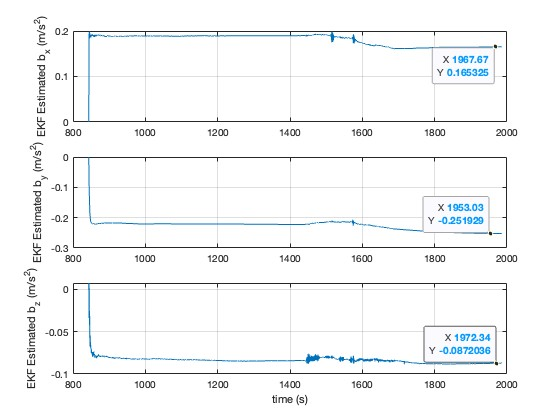
\includegraphics[width=1.6\linewidth]{EKF/EKF_Acb.jpg}  
    \label{fig:EKFAcb}
    \captionsetup{justification=centering} % Ensure caption is centered
    \captionof{figure}{EKF Estimated Accelerometer Bias}
\end{minipage}
\hfill
\begin{minipage}{0.2\textwidth}
    \centering
    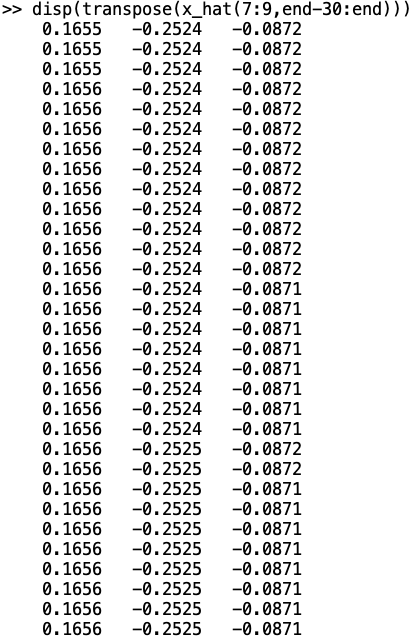
\includegraphics[width=1.6\linewidth]{EKF/AC_Bias.png}  
    \label{fig:Bias}
    \captionsetup{justification=centering} % Ensure caption is centered
    \captionof{figure}{Bias Convergence}
\end{minipage}\\

\textbf{If considering accelerometer bias is not a constant but gradually drifts over time, how will you modify the implementation of EKF to address this issue?}\\

1. The first step would be to augment the state vector to include the bias, which we have done currently.\\

2. The second step would be to model the bias dynamics assuming that it is a random walk, meaning that the bias would change over time with some associated process noise. For this, we would want to build a dynamic model as:
\begin{align*}
\mathbf{b}_{k+1} = \mathbf{b}_k + \mathbf{w}_b
\end{align*}
Where $w_b$ would be your process noise for bias.\\

3. The third step would be to update the measurement model by assuming that the accelerometer measurements are being affected by the true acceleration and the bias, making sure that the measurement model would account for the bias. This measurement model would be included in the H measurement matrix. Therefore if we denote the accelerometer measurement as $ac_k$, the model would become:
\begin{align*}
\mathbf{ac}_k = \mathbf{a}_k + \mathbf{b}_k + \mathbf{v}_k,
\end{align*}
where $a_k$ is the true acceleration of the UAV, $b_k$ is the accelerometer bias, and $v_k$ is the measurement noise.\\

4. The fourth step would be to tune the filter, since bias drift brings in additional uncertainty. Therefore we need to tune the process noise covariance (Q), such that if the noise for the bias is too low, then the filter would be too slow to adapt with the changes in bias, and if it is too high, then the filter could over correct to small noise fluctuations.\\

Implementing these 4 steps would help account for gradual drift in accelerometer bias, and would help modify the implementation of EKF to address these issues.




\section{Conclusion}
\label{Conclusion}
From our NED position derived from raw GPS measurements and our EKF estimated position and velocity, we can analyze the accuracy of the measurements. GPS converted to NED provides us with absolute position, which is extremely useful over a long period of time for long-term accuracy, since it does not drift over time, it provides a consistent positioning based on the signals it receives from the satellite. Furthermore, since GPS has low long-term drift, it provides more accurate positioning. On the other hand, GPS is also prone to noise and can be delayed with a low update rate of only a few Hz which makes it less suitable for UAVs that require real-time high-frequency updates to the data. EKF estimated position and velocity fuse both IMU measurements and GPS measurements providing a filtered estimate with high update rates of a few 100 Hz to allow the EKF to update the position at a faster rate than GPS. Since the EKF accounts for sensor drift, it is able to adjust the position estimate accordingly and smooth out noisy GPS measurements. Our data shows that EKF provided a better estimate of the position and velocity of the UAV, with velocity being less noisy as seen from the graph and the position estimate being identical to what was provided from the NED positions obtained from GPS raw measurements. We were able to see that the UAV took off and landed twice, with the first flight being approximately 10 m in height, and the second flight being approximately 31 m in height. The accelerometer bias converged to $b_x$ converging to
0.164 $m/s^2$, $b_y$ converging to -0.252 $m/s^2$, and $b_z$ converging to -0.087 $m/s^2$. The report shows a successful implementation of an extended kalman filter to better estimate the position and velocity of the UAV in flight.

\section*{Acknowledgments}
\label{Acknowledgements}
1. Parthiv Kukadia would like to thank Professor Wang Fei for the necessary steps to conduct a coordinate transformation from GPS to ECEF to NED position and also for the theory behind implementing an extended Kalman filter.\\

2. Parthiv Kukadia would like to thank TA Yongzhou Pan for clarifying doubts regarding the theoretical implementation of EKF (e.g., the meaning of the Q matrix).

\section*{References}
1. Wang, F. (2024, Aug 4). "3. UAV GPS INS Navigation" [PDF]. National University of Singapore. https://canvas.nus.edu.sg/courses/62933

%\section*{Complete Code}
%\label{Code}
%\begin{lstlisting}
%% Clear past plots, variables and console prints
close all; clear all; clc;

% Load data 
load 'EE5114_CA1.mat';

 %% Accelerometer plot
figure; set(gcf,'numbertitle','off','name','Acceleration');  
subplot(3,1,1); plot(t, acx, 'b'); ylim([-2 2]); ylabel('acx (m/s^2)'); grid on; 
subplot(3,1,2); plot(t, acy, 'b'); ylim([-2 2]); ylabel('acy (m/s^2)'); grid on; 
subplot(3,1,3); plot(t, acz, 'b'); ylabel('acz (m/s^2)'); xlabel('time (s)'); grid on; 

%% Euler angles plot
figure; set(gcf,'numbertitle','off','name','Euler Angles');  
subplot(3,1,1); plot(t, rad2deg(phi), 'b'); ylabel('Roll (degree)'); grid on; 
subplot(3,1,2); plot(t, rad2deg(tht), 'b'); ylabel('Pitch (degree)'); grid on; 
subplot(3,1,3); plot(t, rad2deg(psi), 'b'); ylabel('Yaw (degree)'); xlabel('time (s)'); grid on; 


%% GPS plot
figure; set(gcf,'numbertitle','off','name','GPS');  
subplot(3,2,1); plot(t, lon); ylabel('Longitude'); grid on;
subplot(3,2,3); plot(t, lat); ylabel('Latitude'); grid on;
subplot(3,2,5); plot(t, alt); ylabel('Altitude'); grid on; xlabel('time (s)');

subplot(3,2,2); plot(t, gps_nSat, '.'); ylabel('Sat'); grid on;
subplot(3,2,4); plot(t, eph); ylabel('Eph'); grid on; ylim([0 5]);
subplot(3,2,6); plot(t, epv); ylabel('Epv'); grid on; ylim([0 5]); xlabel('time (s)');

%% Motor signal plot
figure; set(gcf,'numbertitle','off','name','Motor Signal');  
hold on;
plot(t,out1,'r');
plot(t,out2,'g');
plot(t,out3,'b');
plot(t,out4,'y');
legend('Motor1','Motor2','Motor3','Motor4'); 
ylabel('Motor inputs'); xlabel('time (s)'); ylim([1000 2000]); grid on;

%%%%%%%%% Your own coding work start from here %%%%%%%%%%%

%% Convert GPS raw measurements to local NED position values
% To convert GPS to Local NED, need to convert Geodetic to ECEF to NED

% Convert Latitude and Longitude to Radians
lat_rad = deg2rad(lat);
lon_rad = deg2rad(lon);

% Create a function to convert GPS to NED coordinate Frame
function [NED_Coordinates] = GPStoNED(lat_rad, lon_rad, alt)

    % Constants for Earth Ellipsoid to convert from Geodetic to ECEF
    a = 6378137;
    b = 6356752.3142;
    e2 = 1 - (b^2 / a^2);

    % Define initial UAV position as reference position
    lat_0 = lat_rad(1); % Reference Latitude
    lon_0 = lon_rad(1); % Reference Longitude
    alt_0 = alt(1); % Reference Altitude

    % Convert defined intial GPS reference position to ECEF coordinate frame
    [x_e0, y_e0, z_e0] = GPStoECEF(lat_0, lon_0, alt_0, a, e2);

    % Create arrays for NED Coordinates to be stored after iteration
    NED_Coordinates = zeros(length(lat_rad), 3);

    % Loop over all GPS raw measurements and convert each to NED coordinates
    for i = 1:length(lat_rad)
        % Convert GPS raw measurements to ECEF coordinate frame
        [x_e, y_e, z_e] = GPStoECEF(lat_rad(i), lon_rad(i), alt(i), a, e2);
        
        % Convert ECEF measurements to NED coordinate frame
        [x_n, y_n, z_n] = ECEFtoNED(x_e, y_e, z_e, x_e0, y_e0, z_e0, lat_rad(i), lon_rad(i));

        % Store NED coordinates in created arrays
        NED_Coordinates(i, :) = [x_n, y_n, z_n];
    end

end

% Create a function to convert GPS to ECEF coordinate frame
function [x_e, y_e, z_e] = GPStoECEF(lat, lon, alt, a, e2)
    % Define radius of curvature
    N = a ./ sqrt(1 - e2 .* sin(lat).^2); % Radius of curvature

    % Convert GPS raw measurements to ECEF coordinate frame
    x_e = (N + alt) .* cos(lat) .* cos(lon);
    y_e = (N + alt) .* cos(lat) .* sin(lon);
    z_e = ((1 - e2) .* N + alt) .* sin(lat);
end

% Create a function to convert ECEF to NED coordinate frame
function [x_n, y_n, z_n] = ECEFtoNED(x_e, y_e, z_e, x_e0, y_e0, z_e0, lat, lon)
    
    % Difference between ECEF current coordinate and ECEF reference point
    dx = x_e - x_e0;
    dy = y_e - y_e0;
    dz = z_e - z_e0;

    % Rotation matrix to go from ECEF to NED coordinate system
    R = [-sin(lat) * cos(lon), -sin(lon) , -cos(lat) * cos(lon) ;
         -sin(lat) * sin(lon), cos(lon)  , -cos(lat) * sin(lon) ;
         cos(lat)            ,     0     , -sin(lat)           ];
    
    % Calculate NED coordinates
    NED = R' * [dx; dy; dz];
    x_n = NED(1); y_n = NED(2); z_n = NED(3);
end

% Run the NED_Coordinates function to compute a GPS to NED Coordinate
% Transform and substitute into correct naming convention [x_n, y_n, z_n]
[NED_coords] = GPStoNED(lat_rad, lon_rad, alt);
x_n = NED_coords(:,1); y_n = NED_coords(:,2); z_n = NED_coords(:,3);

%% Implement EKF to estimate NED position and velocity
% Implementing EKF for time 2nd UAV take-off and landing where t_min is 
% 10 minutes before UAV taking off and t_max is 5 minutes after landing
% From Motor Signal, we can see that UAV took off at 1440 seconds,
% and landed at 1695 seconds

% Define time interval as provided in problem statement and define time
% index to synchronize data between GPS and IMU to align readings based on
% timestamp
start_t = 1443 - 600; % 10 min before taking-off a second time
start_i = find(t>= start_t,1); % Start time index
end_t = 1685 + 300; % 5 min after landing a second time
end_i = find(t>= end_t,1); % End time index
time_int = t(start_i:end_i); % Define time values from time dataset

% State Variables of interest [NED Position, NED Velocity, Accelerometer Bias]
% x = [x_n, y_n, z_n, v_x, v_y, v_z, b_x, b_y, b_z]
% Define initial state, covariance, and measurement noise covariance
x0 = [x_n(start_i); y_n(start_i); z_n(start_i); 0; 0; 0; 0; 0; 0]; % State
P0 = eye(9); % Covariance
R = diag([eph,eph,epv]) * 1e-3; % Measurement noise covariance - most reliable is GPS
x_hat = zeros(9, length(time_int)); % Create arrays for NED estimate coordinates

% System Matrices
for i = start_i:end_i
    
    dt = (time_int(end) - time_int(1))/(length(time_int)); % Assuming uniform sampling

    % Create Rotation Matrix to move from NED to Ground Frame
    R_NEDtoGround = [cos(psi(i)) * cos(tht(i)) , (cos(psi(i)) * sin(tht(i)) * sin(phi(i))) - (sin(psi(i)) * cos(phi(i))) , (cos(psi(i)) * sin(tht(i)) * cos(phi(i))) + (sin(psi(i)) * sin(phi(i)));
                     sin(psi(i)) * cos(tht(i)) , (sin(psi(i)) * sin(tht(i)) * sin(phi(i))) + (cos(psi(i)) * cos(phi(i))) , (sin(psi(i)) * sin(tht(i)) * cos(phi(i))) - (cos(psi(i)) * sin(phi(i)));
                     -sin(tht(i))              ,  cos(tht(i)) * sin(phi(i))                                              ,  cos(tht(i)) * cos(phi(i))                                            ];
    
    % Create the State Transition Matrix
    F_1 = [eye(3)     , diag([dt, dt, dt]) , diag([(-dt^2)/2, (-dt^2)/2, (-dt^2)/2]);
           zeros(3,3) , eye(3)             , diag([-dt, -dt, -dt])                 ];
    F_2 = [eye(6)     , zeros(6,3)    ;
           zeros(3,6) , R_NEDtoGround];
    F = [F_1 * F_2         ;  % Upper region of F
         zeros(3,6), eye(3)]; % Lower region of F

    % Define gravity for G matrix
    g = 9.81; % m/s^2

    % Create the Control Input Matrix
    G_1 = [diag([(dt^2)/2, (dt^2)/2 , (dt^2)/2]);
           diag([  dt    ,    dt    ,   dt    ]);
                          zeros(3,3)           ];
    G_2 = [R_NEDtoGround, [0 ; 0 ; g]];
    G = G_1 * G_2;

    % Create process noise covariance matrix
    Q = G * diag([0.7 , 0.4 , 1.5 , 0]) * G'; %qx, qy, qz

    % Prediction Step - using previous time step to produce estimation of
    % state at current time step
    x_pred = (F * x0) + (G * [acx(i) ; acy(i) ; acz(i) ; 1]);
    P_pred = (F * P0 * F') + Q;

    % Defining the Measurement Model of GPS
    y = [x_n(i+1) ; y_n(i+1) ; z_n(i+1)];

    % To account for difference in GPS update rate and IMU update rate,
    % need to input a condition such that GPS update rate is lower to
    % provide long-term position accuracy
        if mod(i, 2) == 0
            % Correction Step with GPS update (every 3rd iteration)
            H = [eye(3), zeros(3, 6)]; % Output Matrix
            S = (H * P_pred * H') + R; % Residual covariance
            W = P_pred * H' * inv(S);  % Optimal Kalman Gain

            % Update step using GPS
            x0 = x_pred + (W * (y - (H * x_pred)));
            P0 = (eye(9) - (W * H)) * P_pred;
        
        else
            % Update step without GPS (IMU update)
            x0 = x_pred;
            P0 = P_pred;
        end

    % Store estimates
    x_hat(:,i) = x0;
end   

% Extract estimated velocities
x_hat = x_hat(:,start_i:end_i);
EKF_pos_N = x_hat(1, :);
EKF_pos_E = x_hat(2, :);
EKF_pos_D = x_hat(3, :);
EKF_vel_N = x_hat(4, :);
EKF_vel_E = x_hat(5, :);
EKF_vel_D = x_hat(6, :);
EKF_bx = x_hat(7, :);
EKF_by = x_hat(8, :);
EKF_bz = x_hat(9, :);

% Calculate NED Velocites from GPS Measurement
dt_v = diff(time_int);
v_n = diff(x_n(start_i:end_i))./dt_v;
v_e = diff(y_n(start_i:end_i))./dt_v;
v_d = diff(z_n(start_i:end_i))./dt_v;

% Calculate NED Acceleration from GPS Measurement
dt_a = diff(dt_v);
a_n = diff(v_n)./dt_a;
a_e = diff(v_e)./dt_a;
a_d = diff(v_d)./dt_a;


%% Result plots

%% GPS Plot - Processed
figure; set(gcf,'numbertitle','off','name','GPS');  
subplot(3,2,1); plot(t, lon); title('Pre-Processing GPS Plot'); ylabel('Longitude'); grid on;
subplot(3,2,3); plot(t, lat); ylabel('Latitude'); grid on;
subplot(3,2,5); plot(t, alt); ylabel('Altitude'); grid on; xlabel('time (s)');
subplot(3,2,2); plot(t(125:end), lon(125:end)); title('Post-Processing GPS Plot'); ylabel('Longitude'); grid on;
subplot(3,2,4); plot(t(125:end), lat(125:end)); ylabel('Latitude'); grid on;
subplot(3,2,6); plot(t(125:end), alt(125:end)); ylabel('Altitude'); grid on; xlabel('time (s)');

%% GPS to NED Plot
figure; set(gcf,'numbertitle','off','name','NED Positions from GPS Raw Measurements');  
subplot(3,1,1); plot(t(125:end), x_n(125:end));title('NED Positions from GPS Raw Measurements'); ylabel('North (x_n, m)'); grid on;
subplot(3,1,2); plot(t(125:end), y_n(125:end)); ylabel('East (y_n, m)'); grid on;
subplot(3,1,3); plot(t(125:end), z_n(125:end)); ylabel('Down (z_n, m)'); grid on; xlabel('time (s)');

%% Plot of estimated NED positions based on EKF vs. time
figure; set(gcf,'numbertitle','off','name','EKF Estimated NED Positions');  
subplot(3,1,1); plot(time_int, EKF_pos_N, 'k', time_int, x_n(start_i:end_i), 'r--' ); legend('EKF Estimated', 'NED from GPS'); ylabel('North Position, x_n (m)'); grid on;
subplot(3,1,2); plot(time_int, EKF_pos_E, 'k', time_int, y_n(start_i:end_i), 'r--' ); legend('EKF Estimated', 'NED from GPS'); ylabel('East Position, y_n (m)'); grid on;
subplot(3,1,3); plot(time_int, EKF_pos_D, 'k', time_int, z_n(start_i:end_i), 'r--' ); legend('EKF Estimated', 'NED from GPS'); ylabel('Down Position, z_n (m)'); grid on;
xlabel('time (s)');

%% Estimated NED velocities based on EKF Implementation againt time
figure; set(gcf,'numbertitle','off','name','EKF Estimated NED Velocity');  
subplot(3,1,1); plot(time_int(2:end), v_n, 'r--', time_int, EKF_vel_N, 'k' ); legend('NED from GPS', 'EKF Estimated'); ylabel('North Velocity, v_xn (m/s)'); grid on;
subplot(3,1,2); plot(time_int(2:end), v_e, 'r--', time_int, EKF_vel_E, 'k' ); legend('NED from GPS', 'EKF Estimated'); ylabel('East Velocity, v_yn (m/s)'); grid on;
subplot(3,1,3); plot(time_int(2:end), v_d, 'r--', time_int, EKF_vel_D, 'k'); legend('NED from GPS', 'EKF Estimated'); ylabel('Down Velocity, v_zn (m/s)'); grid on;
xlabel('Time (s)');

%% Plot of Local NED Acceleration being converted from GPS vs. time
figure; set(gcf,'numbertitle','off','name','NED Acceleration from GPS');  
subplot(3,1,1); plot(time_int(3:end), a_n); ylabel('North Acceleration (a_n, m/s^2)'); grid on;
subplot(3,1,2); plot(time_int(3:end), a_e); ylabel('East Acceleration (a_e, m/s^2)'); grid on;
subplot(3,1,3); plot(time_int(3:end), a_d); ylabel('Down Acceleration (a_d, m/s^2)'); grid on;
xlabel('time (s)');

%% Plot of Accelerometer bias from EKF Implementation against time
figure; set(gcf,'numbertitle','off','name','EKF Estimated Accelerometer Bias');  
subplot(3,1,1); plot(time_int, EKF_bx); ylabel('EKF Estimated b_x (m/s^2)'); grid on;
subplot(3,1,2); plot(time_int, EKF_by); ylabel('EKF Estimated b_y (m/s^2)'); grid on;
subplot(3,1,3); plot(time_int, EKF_bz); ylabel('EKF Estimated b_z (m/s^2)'); grid on;
xlabel('time (s)');
\end{lstlisting}
\captionof{figure}{MATLAB Code for Localization Using GPS and IMU Information via EKF Framework}
\label{fig:completecode}



\end{document}
